\documentclass[12pt]{article}

\usepackage{graphicx}

\begin{document}

\title{NavUP - SRS Use Case: Choose Route Type}
\author{SJ du Plooy (12070794)}
\date{\today}
\maketitle


\begin{tabular}{|p{4cm}|p{10cm}|}
\hline

Use Case Element & Description \\
\hline

Use Case Name & 
Choose Route Type \\
\hline

Use Case Description & 
The user must be able to pick from a selection of route types, be it shortest, fastest, wheelchair friendly etc.   \\
\hline

Primary Actor & 
Student/staff/guest \\
\hline

Precondition & 
The user must be within the campus map boundaries and have an active Wi-Fi connection.   \\
\hline

Trigger & 
When the user starts the process of requesting navigation instructions.   \\
\hline

Basic Flow & 
When the user is in the process of setting the conditions needed for navigation, the user will be able to:
\begin{enumerate}
\item Tap on the “Choose Route Type” drop down menu
\item Select the most appropriate option such as
	\begin{enumerate}
	\item Shortest path (Making use of actual distance from point A to B)
	\item Fastest path (Making use of heat maps to plot least congested path from point A to B)
	\item Wheelchair Friendly (Taking to account routs with Elevators and wheelchair ramps available)
	\end{enumerate}
\end{enumerate} \\
\hline

\hline
\end{tabular}


\begin{figure}

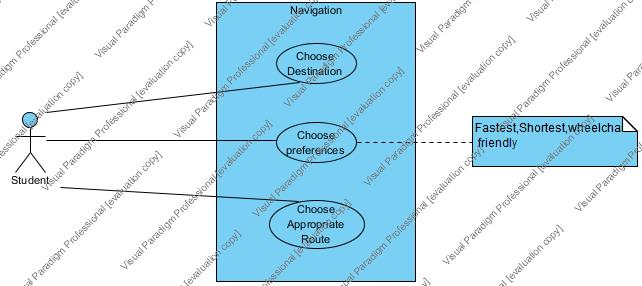
\includegraphics[width=\linewidth]{UseCaseDiagram_ChooseRouteType.jpg}
\caption{Use Case Diagram of the Choose Route Type Use Case.}
\label{fig:UCD1}

\end{figure}

Figure \ref{fig:UCD1} Choose Route Type Use Case Diagram

\end{document}
